% Options for packages loaded elsewhere
\PassOptionsToPackage{unicode}{hyperref}
\PassOptionsToPackage{hyphens}{url}
%
\documentclass[
]{book}
\usepackage{amsmath,amssymb}
\usepackage{lmodern}
\usepackage{iftex}
\ifPDFTeX
  \usepackage[T1]{fontenc}
  \usepackage[utf8]{inputenc}
  \usepackage{textcomp} % provide euro and other symbols
\else % if luatex or xetex
  \usepackage{unicode-math}
  \defaultfontfeatures{Scale=MatchLowercase}
  \defaultfontfeatures[\rmfamily]{Ligatures=TeX,Scale=1}
\fi
% Use upquote if available, for straight quotes in verbatim environments
\IfFileExists{upquote.sty}{\usepackage{upquote}}{}
\IfFileExists{microtype.sty}{% use microtype if available
  \usepackage[]{microtype}
  \UseMicrotypeSet[protrusion]{basicmath} % disable protrusion for tt fonts
}{}
\makeatletter
\@ifundefined{KOMAClassName}{% if non-KOMA class
  \IfFileExists{parskip.sty}{%
    \usepackage{parskip}
  }{% else
    \setlength{\parindent}{0pt}
    \setlength{\parskip}{6pt plus 2pt minus 1pt}}
}{% if KOMA class
  \KOMAoptions{parskip=half}}
\makeatother
\usepackage{xcolor}
\IfFileExists{xurl.sty}{\usepackage{xurl}}{} % add URL line breaks if available
\IfFileExists{bookmark.sty}{\usepackage{bookmark}}{\usepackage{hyperref}}
\hypersetup{
  pdftitle={BioSci 1540: Computational Biology},
  pdfauthor={Nathan L. Brouwer},
  hidelinks,
  pdfcreator={LaTeX via pandoc}}
\urlstyle{same} % disable monospaced font for URLs
\usepackage{color}
\usepackage{fancyvrb}
\newcommand{\VerbBar}{|}
\newcommand{\VERB}{\Verb[commandchars=\\\{\}]}
\DefineVerbatimEnvironment{Highlighting}{Verbatim}{commandchars=\\\{\}}
% Add ',fontsize=\small' for more characters per line
\usepackage{framed}
\definecolor{shadecolor}{RGB}{248,248,248}
\newenvironment{Shaded}{\begin{snugshade}}{\end{snugshade}}
\newcommand{\AlertTok}[1]{\textcolor[rgb]{0.94,0.16,0.16}{#1}}
\newcommand{\AnnotationTok}[1]{\textcolor[rgb]{0.56,0.35,0.01}{\textbf{\textit{#1}}}}
\newcommand{\AttributeTok}[1]{\textcolor[rgb]{0.77,0.63,0.00}{#1}}
\newcommand{\BaseNTok}[1]{\textcolor[rgb]{0.00,0.00,0.81}{#1}}
\newcommand{\BuiltInTok}[1]{#1}
\newcommand{\CharTok}[1]{\textcolor[rgb]{0.31,0.60,0.02}{#1}}
\newcommand{\CommentTok}[1]{\textcolor[rgb]{0.56,0.35,0.01}{\textit{#1}}}
\newcommand{\CommentVarTok}[1]{\textcolor[rgb]{0.56,0.35,0.01}{\textbf{\textit{#1}}}}
\newcommand{\ConstantTok}[1]{\textcolor[rgb]{0.00,0.00,0.00}{#1}}
\newcommand{\ControlFlowTok}[1]{\textcolor[rgb]{0.13,0.29,0.53}{\textbf{#1}}}
\newcommand{\DataTypeTok}[1]{\textcolor[rgb]{0.13,0.29,0.53}{#1}}
\newcommand{\DecValTok}[1]{\textcolor[rgb]{0.00,0.00,0.81}{#1}}
\newcommand{\DocumentationTok}[1]{\textcolor[rgb]{0.56,0.35,0.01}{\textbf{\textit{#1}}}}
\newcommand{\ErrorTok}[1]{\textcolor[rgb]{0.64,0.00,0.00}{\textbf{#1}}}
\newcommand{\ExtensionTok}[1]{#1}
\newcommand{\FloatTok}[1]{\textcolor[rgb]{0.00,0.00,0.81}{#1}}
\newcommand{\FunctionTok}[1]{\textcolor[rgb]{0.00,0.00,0.00}{#1}}
\newcommand{\ImportTok}[1]{#1}
\newcommand{\InformationTok}[1]{\textcolor[rgb]{0.56,0.35,0.01}{\textbf{\textit{#1}}}}
\newcommand{\KeywordTok}[1]{\textcolor[rgb]{0.13,0.29,0.53}{\textbf{#1}}}
\newcommand{\NormalTok}[1]{#1}
\newcommand{\OperatorTok}[1]{\textcolor[rgb]{0.81,0.36,0.00}{\textbf{#1}}}
\newcommand{\OtherTok}[1]{\textcolor[rgb]{0.56,0.35,0.01}{#1}}
\newcommand{\PreprocessorTok}[1]{\textcolor[rgb]{0.56,0.35,0.01}{\textit{#1}}}
\newcommand{\RegionMarkerTok}[1]{#1}
\newcommand{\SpecialCharTok}[1]{\textcolor[rgb]{0.00,0.00,0.00}{#1}}
\newcommand{\SpecialStringTok}[1]{\textcolor[rgb]{0.31,0.60,0.02}{#1}}
\newcommand{\StringTok}[1]{\textcolor[rgb]{0.31,0.60,0.02}{#1}}
\newcommand{\VariableTok}[1]{\textcolor[rgb]{0.00,0.00,0.00}{#1}}
\newcommand{\VerbatimStringTok}[1]{\textcolor[rgb]{0.31,0.60,0.02}{#1}}
\newcommand{\WarningTok}[1]{\textcolor[rgb]{0.56,0.35,0.01}{\textbf{\textit{#1}}}}
\usepackage{longtable,booktabs,array}
\usepackage{calc} % for calculating minipage widths
% Correct order of tables after \paragraph or \subparagraph
\usepackage{etoolbox}
\makeatletter
\patchcmd\longtable{\par}{\if@noskipsec\mbox{}\fi\par}{}{}
\makeatother
% Allow footnotes in longtable head/foot
\IfFileExists{footnotehyper.sty}{\usepackage{footnotehyper}}{\usepackage{footnote}}
\makesavenoteenv{longtable}
\usepackage{graphicx}
\makeatletter
\def\maxwidth{\ifdim\Gin@nat@width>\linewidth\linewidth\else\Gin@nat@width\fi}
\def\maxheight{\ifdim\Gin@nat@height>\textheight\textheight\else\Gin@nat@height\fi}
\makeatother
% Scale images if necessary, so that they will not overflow the page
% margins by default, and it is still possible to overwrite the defaults
% using explicit options in \includegraphics[width, height, ...]{}
\setkeys{Gin}{width=\maxwidth,height=\maxheight,keepaspectratio}
% Set default figure placement to htbp
\makeatletter
\def\fps@figure{htbp}
\makeatother
\setlength{\emergencystretch}{3em} % prevent overfull lines
\providecommand{\tightlist}{%
  \setlength{\itemsep}{0pt}\setlength{\parskip}{0pt}}
\setcounter{secnumdepth}{5}
\usepackage{booktabs}
\ifLuaTeX
  \usepackage{selnolig}  % disable illegal ligatures
\fi
\usepackage[]{natbib}
\bibliographystyle{apalike}

\title{BioSci 1540: Computational Biology}
\author{Nathan L. Brouwer}
\date{2021-09-01}

\begin{document}
\maketitle

{
\setcounter{tocdepth}{1}
\tableofcontents
}
\hypertarget{welcome}{%
\chapter{Welcome}\label{welcome}}

This is the syllabus.

\begin{Shaded}
\begin{Highlighting}[]
\FunctionTok{install.packages}\NormalTok{(}\StringTok{"bookdown"}\NormalTok{)}
\CommentTok{\# or the development version}
\CommentTok{\# devtools::install\_github("rstudio/bookdown")}
\end{Highlighting}
\end{Shaded}

\hypertarget{intro}{%
\chapter{Introduction}\label{intro}}

\textbf{This is the syllabus for BIOSCI 1540: Computational Biology.}

This is both the first course in the core sequence of classes of the Computational Biology major and also an elective for most Biological Sciences majors.

This syllabus contains both key course policies and also is a repository for useful information about computational biology.

The first several pages contain key information about the course. Subsequent pages are organized alphabetically by major topic.

Pages marked ``Appendix'' are additional information about computational biology or research that you may find useful.

Your first assignment in the class will be to read through the syllabus and complete a ``Syllabus treasure hunt'' assignment on Canvas.

If you have a question about the syllabus (after you complete the syllabus treasure hunt) or even just spot a typo, post a comment on \href{https://github.com/brouwern/BIOSCI_1540}{GitHub} at \url{https://github.com/brouwern/BIOSCI_1540}

You'll be shown how to add comments on GitHub in class. The next page of the syllabus is a page for practicing adding comments.

\hypertarget{github-comments-practice}{%
\chapter{Github comments practice}\label{github-comments-practice}}

Scroll down and locate the heading for the leter your last name begins with. Then locate the bullet point for theletter your first name begins with and add a comment to that line of code.

If you intials do not appear add a comment to the ``other'' label.

\hypertarget{a}{%
\section{A}\label{a}}

\begin{itemize}
\tightlist
\item
  E
\item
  J
\item
  other
\end{itemize}

\hypertarget{b}{%
\section{B}\label{b}}

\begin{itemize}
\tightlist
\item
  A
\item
  H
\item
  L
\item
  M
\item
  O
\item
  S
\item
  other
\end{itemize}

\hypertarget{c}{%
\section{C}\label{c}}

\begin{itemize}
\tightlist
\item
  E
\item
  J
\item
  M
\item
  R
\item
  Z
\item
  other
\end{itemize}

\hypertarget{d}{%
\section{D}\label{d}}

\begin{itemize}
\tightlist
\item
  D
\item
  J
\item
  K
\item
  L
\item
  La
\item
  Le
\item
  Li
\item
  Lo
\item
  R
\item
  other
\end{itemize}

\hypertarget{e}{%
\section{E}\label{e}}

\begin{itemize}
\tightlist
\item
  Z
\item
  other
\end{itemize}

\hypertarget{f}{%
\section{F}\label{f}}

\begin{itemize}
\tightlist
\item
  C
\item
  G
\item
  L
\item
  Z
\item
  other
\end{itemize}

\hypertarget{g}{%
\section{G}\label{g}}

\begin{itemize}
\tightlist
\item
  E
\item
  J
\item
  M
\item
  S
\item
  other
\end{itemize}

\hypertarget{h}{%
\section{H}\label{h}}

\begin{itemize}
\tightlist
\item
  D
\item
  Ja
\item
  Je
\item
  Ji
\item
  Jo
\item
  S
\item
  other
\end{itemize}

\hypertarget{j}{%
\section{J}\label{j}}

\begin{itemize}
\tightlist
\item
  V
\item
  other
\end{itemize}

\hypertarget{k}{%
\section{K}\label{k}}

\begin{itemize}
\tightlist
\item
  M
\item
  other
\end{itemize}

\hypertarget{m}{%
\section{M}\label{m}}

\begin{itemize}
\tightlist
\item
  G
\item
  C
\item
  N
\item
  Na
\item
  Ne
\item
  Ni
\item
  S
\item
  other
\end{itemize}

\hypertarget{n}{%
\section{N}\label{n}}

\begin{itemize}
\tightlist
\item
  M
\item
  other
\end{itemize}

\hypertarget{n-1}{%
\section{N}\label{n-1}}

\begin{itemize}
\tightlist
\item
  N
\item
  other
\end{itemize}

\hypertarget{p}{%
\section{P}\label{p}}

\begin{itemize}
\tightlist
\item
  C
\item
  J
\item
  H
\item
  S
\item
  other
\end{itemize}

\hypertarget{p-1}{%
\section{P}\label{p-1}}

\begin{itemize}
\tightlist
\item
  J
\item
  other
\end{itemize}

\hypertarget{r}{%
\section{R}\label{r}}

\begin{itemize}
\tightlist
\item
  A
\item
  C
\item
  R
\item
  Ra
\item
  Re
\item
  Ri
\item
  Ro
\item
  V
\item
  Va
\item
  Ve
\item
  Vi
\item
  other
\end{itemize}

\hypertarget{s}{%
\section{S}\label{s}}

\begin{itemize}
\tightlist
\item
  A
\item
  B
\item
  D
\item
  E
\item
  En
\item
  Er
\item
  I
\item
  J
\item
  S
\item
  V
\item
  Va
\item
  Ve
\item
  Vi
\item
  Vo
\item
  other
\end{itemize}

\hypertarget{t}{%
\section{T}\label{t}}

\begin{itemize}
\tightlist
\item
  A
\item
  other
\end{itemize}

\hypertarget{v}{%
\section{V}\label{v}}

\begin{itemize}
\tightlist
\item
  T
\item
  Ta
\item
  Ti
\item
  Te
\item
  To
\item
  other
\end{itemize}

\hypertarget{w}{%
\section{W}\label{w}}

\begin{itemize}
\tightlist
\item
  A
\item
  G
\item
  other
\end{itemize}

\hypertarget{x}{%
\section{X}\label{x}}

\begin{itemize}
\tightlist
\item
  X
\item
  other
\end{itemize}

\hypertarget{y}{%
\section{Y}\label{y}}

\begin{itemize}
\tightlist
\item
  H
\item
  S
\item
  X
\item
  other
\end{itemize}

\hypertarget{z}{%
\section{Z}\label{z}}

\begin{itemize}
\tightlist
\item
  Y
\item
  other
\end{itemize}

\hypertarget{meeting-times}{%
\chapter{Meeting times}\label{meeting-times}}

The course will meeting in-person on Tuesdays and Thursday.

\textbf{Location:} 1502 \href{https://www.tour.pitt.edu/tour/wesley-w-posvar-hall}{Posvar Hall}
\textbf{Days:} Tuesday \& Thursday\\
\textbf{Times:} 4:00PM - 5:15PM
Aug 31, 2021-Dec 10, 2021

The first two weeks all lectures will be live-streamed on \href{https://pitt.zoom.us/j/99372114800}{Zoom}: \url{https://pitt.zoom.us/j/99372114800}\\
Password: ``BLOSUM''

There is no recitation for this course.

The official Pitt \textbf{Academic Calendar} can be found {[}here{]}(\url{https://catalog.upp.pitt.edu/mime/media/212/3179/Academic+Calendar+2021-2022.pdf}: \url{https://catalog.upp.pitt.edu/mime/media/212/3179/Academic+Calendar+2021-2022.pdf}

\hypertarget{nlb}{%
\chapter{Instructor}\label{nlb}}

\textbf{Nathan L. Brouwer}, PhD
Office: Langley Hall 215A\\
(In the former Neuroscience office suite)\\
Email: nlb24 at pitt.edu\\
Github: \url{https://github.com/brouwern}

\hypertarget{academic-integrity}{%
\chapter{Academic integrity}\label{academic-integrity}}

Dr.~Brouwer, the Bio Sci department, and the University all take academic integrity very seriously. Cheating includes any form of plagiarism, including copying other students' work or using other resources without proper attribution.

\begin{enumerate}
\def\labelenumi{\arabic{enumi}.}
\tightlist
\item
  If you are caught cheating on a graded assignment, you will receive a zero on the assignment.
\item
  If you are caught cheating on an exam, you will receive a zero on the exam, an F in the course, and an Academic Integrity Violation Report will be filed.
\end{enumerate}

Below is the University's Policy on Academic Integrity:

\begin{quote}
``Students in this course are expected to comply with the University of Pittsburgh School of Arts \& Sciences Academic Integrity Code located at www.as.pitt.edu/faculty/policy/integrity.html. Any student suspected of failing to meet the student obligations of the code during the semester will be required to participate in the procedures for adjudication, initiated at the instructor level. This may include, but is not limited to, confiscation of the assignment of any individual suspected of violating the code. A minimum sanction of a zero score for the assignment will be imposed. Violation of the Academic Integrity Code requires the instructor to submit an Academic Integrity Violation Report to the Dean.''
\end{quote}

\hypertarget{assessments}{%
\chapter{Assessments Overview}\label{assessments}}

The primary form of assessment in the course will be 5 unit tests.

The final is the 5th unit test, but will also draw on themes from throughout the semester

Other forms of assessment will include,\\
1. \textbf{Test revisions} (aka Test Reworks), which will count as a form of homework and do not add points back to your test.\\
1. \textbf{Canvas Quiz questions} related to lecture videos, \textbf{Code checkpoints} to assure that you can execute key functions, and \textbf{Software checkpoints} to assure that you have the proper software involved.
1. Additional homework
1. Practice tests or test preparation assignments.

\hypertarget{test-taking-policies}{%
\section{Test-taking policies}\label{test-taking-policies}}

Tests will be in-person during the regularly schedule time and administered as a combination of

\begin{enumerate}
\def\labelenumi{\arabic{enumi}.}
\tightlist
\item
  Stand-alone canvas quiz questions
\item
  Canvas quiz questions based on code I provide
\item
  Code-based questions which you'll answer via a separtate file, submitted via Canvas.
\end{enumerate}

\hypertarget{key-test-policies}{%
\section{Key test policies}\label{key-test-policies}}

\begin{enumerate}
\def\labelenumi{\arabic{enumi}.}
\tightlist
\item
  All answers will be submitted by the end of the normal class period.\\
\item
  If you are unable to take or complete an exam your score will be eligible to be dropped or replaced as specified elsewhere in the syllabus.
\item
  It is your responsibility to assure that you have adequate power in your devices and internet access to complete exams.\\
\item
  Adjustments will be made as necessary for students with DRS accommodations.
\item
  You may not communicate with other students while taking a test.
\end{enumerate}

\hypertarget{test-dropping-policy}{%
\section{Test dropping policy}\label{test-dropping-policy}}

Your lowest unit test will be dropped. Your second-lowest score can be replaced by the final, if you score higher on the final. See the section on the final exam for further explanation.

\hypertarget{final-exam-policies}{%
\section{Final Exam Policies}\label{final-exam-policies}}

The final will cover conceptual material covered after the Unit 4 test. You will also need to draw on R skills from throughout the semester.

The final exam will \ldots{}
1, Take place during finals week on the day scheduled by the University
1. Is required
1. Follow the general format of other tests.

The final exam is required and will be scheduled as per the University calendar.

As noted elsewhere your lowest test score will be automatically dropped and your score for tests calculated based on your 3 best tests. Additionally, I will compare your performance on the final to those three tests and if your score on the final is higher then I will upgrade that score to your score on the final. Your final eaxm can therefore contribute to you score in 2 ways - as the final, and as a replacement of your second lowest of the 4 unit tests. Therefore, one of your exams is always dropped, and a second one is potentially replaced.

\hypertarget{exam-buffer-question-policy}{%
\section{Exam ``buffer question'' policy}\label{exam-buffer-question-policy}}

The unit tests and the final exam will have 1 to 2 ``buffer points.'' The way this work is that there will be, for example, 26 questions but the test will be worth a maximum of 25 points. The maximum score on the test will be capped at 25 points. If you miss 1 question you will get 25/25 points instead of 25/26. If you miss two questions you will get 24/25 and so forth. Scores greater than 100\% will not be given.

\hypertarget{homework}{%
\chapter{Assessments - Homework policies}\label{homework}}

Homework for outside of class will be assigned via Canvas.

\textbf{Late assignments:} Canvas will automatically deduct 0.5\% of your score on all non-test assignments per hour, rounding to the nearest hour (12\%/day). 29 minutes = 0 hours = full credit, 31 minutes = 1 hour.

\hypertarget{course-communication---overview}{%
\chapter{Course communication - Overview}\label{course-communication---overview}}

\hypertarget{primary-modes-of-communication}{%
\section{Primary modes of communication}\label{primary-modes-of-communication}}

All important details will be sent via Canvas messages and mentioned/discussed in class. It is your responsibility to regularly check Canvas messages to stay abreast of the course. Most communication will occur on Fridays, but important updates may be sent out at other times.

\hypertarget{secondary-modes-of-communication}{%
\section{Secondary modes of communication}\label{secondary-modes-of-communication}}

\hypertarget{github-issues}{%
\subsection{Github ``issues''}\label{github-issues}}

In this class we will be making extensive use of the code management site \href{https://github.com/}{GitHub}. Most communication about homework and other assignments will occur via GitHub's \href{https://guides.github.com/features/issues/}{Issues}{]} feature. In particular, to foster discussion we will use GitHub Issues to create forums around assignments and you will be required to submit comments.

\hypertarget{microsoft-sharepoint}{%
\subsection{Microsoft SharePoint}\label{microsoft-sharepoint}}

Files containing code for this course will be distributed using Microsoft Sharepoint. Sharepoint has messaging features which I may pilot test but will not rely on.

\hypertarget{email_and_canvas_msg}{%
\chapter{Course communication - Email and Canvas Messages}\label{email_and_canvas_msg}}

Announcements to the whole course via Canvas will occur typically on \textbf{Friday} afternoons. Other communication related to course administration will also occur via Canvas messages.

Your can message me on Canvas or email me at nlb24 at pitt.edu.

Please include ``Comp Bio'' as the 1st thing in your email subject line with an informative bit of information as the ``\ldots{}''. e.g.~``Comp Bio 2: problem accessing TopHat''. (Questions related to code are best submitted via GitHub).

If you use another email service as your primary email (eg GMail) please set your Pitt email to forward there.

For info on forwarding your Pitt email to your personal account follow this link: \url{https://bit.ly/2Riz7dx}

I try to answer all emails received on weekdays before 5 pm within 24-36 hrs. Emails received after 5 pm will be answered at the earliest the following morning. Emails received on the weekend will be answered Monday.

Please consult this syllabus before asking questions about course policies and the schedule, and refer to relevant information such as URLs, subject headings or dates. Screengrabs are super helpful. If the entire answer to your question can be found in the syllabus I will likely respond by saying ``\emph{This is in the syllabus, Cheers, Dr.~B.}''.

Questions relevant to the whole class may be reposted (with identifying details removed) to Canvas.

\hypertarget{communication---university-email-policy}{%
\chapter{Communication - University email policy}\label{communication---university-email-policy}}

Each student is issued a University e-mail address (username at pitt.edu). This e-mail address may be used by the University for official communication. Students are expected to read e-mail sent to this account on a regular basis. Failure to read and react to University communications in a timely manner does not absolve the student from knowing and complying with the content of the communications.

The University provides an e-mail forwarding service that allows students to read their e-mail via other service providers. Students that choose to forward their e-mail from their pitt.edu address to another address do so at their own risk. If e-mail is lost as a result of forwarding, it does not absolve the student from responding to official communications sent to their University e-mail address.

To forward e-mail sent to your University account, go to \url{http://accounts.pitt.edu}, log into your account, click on Edit Forwarding Addresses, and follow the instructions on the page. Be sure to log out of your account when you have finished.

For the full E-mail Communication Policy, go to bc.pitt.edu/policies/policy/09/09-10-01.html.

\hypertarget{catalog-description}{%
\chapter{Catalog description}\label{catalog-description}}

The catalog description of this course is:

\begin{quote}
``This course is designed to give students a broad understanding of how computational approaches can be used to solve problems in biology. Both the biological and computational underpinnings of the methods will be addressed.''
\end{quote}

\hypertarget{course-materials-overview}{%
\chapter{Course materials overview}\label{course-materials-overview}}

Thanks to an Open Educational Resources (OER) grant from The Office of the Provost, there are no books to buy for this course - all course materials are free and will be provided digitally through Canvas.

Reading will take several forms:

\begin{enumerate}
\def\labelenumi{\arabic{enumi}.}
\tightlist
\item
  files containing computer code (scripts)
\item
  articles and blog posts,
\item
  textbook readings.
\end{enumerate}

Importantly, we'll be taking a very novel approach to the textbook for this course: \textbf{you will actually be building it yourself!}

Details will be provided in-class, but the gist regarding the textbook is:

\begin{enumerate}
\def\labelenumi{\arabic{enumi}.}
\tightlist
\item
  Most weeks you will be provided 1 or 2 chapters of the book in the form of computer files (``scripts'').
\item
  For homework you will do exercises embedded in the chapters.
\item
  When the exercises are successfully completed you will be able to convert the files to Web Pages and post them to your own Portfolio of book chapters and other completed activities.
\end{enumerate}

\hypertarget{course-materials---software}{%
\chapter{Course materials - Software}\label{course-materials---software}}

Installation and account creation for all software will be covered in detail during class or via assignments and accompanying videos. If you want to get prepared early for the course you can explore these on your own.

For information on getting started with R see \href{https://brouwern.github.io/getRdone/}{Get R Done!}.

\hypertarget{primary-software}{%
\section{Primary software}\label{primary-software}}

\hypertarget{programming-environment-r}{%
\subsection{Programming environment: R}\label{programming-environment-r}}

We will use the open-source language \protect\hyperlink{r}{R})(\url{https://cran.r-project.org/}) for almost everything in this course.

\textbf{NOTE}: If you have used R before that's awesome!

However, \textbf{Please update your installation when the class begins} - R goes through regular updates and works best with the newest version.

If you are having trouble installing R an excellent resource is:
\url{https://learningstatisticswithr.com/book/introR.html}

\textbf{REFERENCE}\\
R Core Team (2021). R: A language and environment for statistical computing. R Foundation for Statistical Computing, Vienna, Austria. www.R-project.org/.

\hypertarget{integrated-developement-environment-ide}{%
\subsection{Integrated developement environment (IDE)}\label{integrated-developement-environment-ide}}

We'll use \href{https://www.rstudio.com/}{RStudio} as the front-end for working with R.

\textbf{NOTE}: If you've use RStudio before please update it when the course begins.

\textbf{{[}RStudio{]}(\url{https://www.rstudio.com/}:} www.rstudio.com/products/rstudio/download/\#download

\hypertarget{cloud-based-r}{%
\subsection{Cloud-based R}\label{cloud-based-r}}

As a back-up to running R on your desktop I'll also introduce you to {[}RStudio Cloud{]}(\url{https://rstudio.cloud/}. There are also several excellent \href{https://rstudio.cloud/learn/primers}{primers} which we'll use.

\textbf{\href{https://rstudio.cloud/}{RStudio cloud}:} \url{https://rstudio.cloud/}

\hypertarget{code-sharing}{%
\section{Code sharing}\label{code-sharing}}

\hypertarget{microsoft-sharepoint-1}{%
\subsection{Microsoft SharePoint}\label{microsoft-sharepoint-1}}

R code and other files will be distributed to you via a personal folder on \textbf{SharePoint}, accessed via your \textbf{OneDrive} account.

You will need to ``sync'' your OneDrive account to your computer desktop to allow me to help you with your work. No code files will be shared via email or Canvas during the course.

\textbf{NOTE}: If you do not have access to a computer you can sync your OneDrive account please contact me so we can workout a system.

\hypertarget{github}{%
\subsection{GitHub}\label{github}}

Most code for this course will be available on \href{https://github.com/}{GitHub} and you will need to create an account for some activities.

Links will be distributed directly to you, but you can also see key resources pinned to my profile at \url{https://github.com/brouwern}

\hypertarget{r-packages}{%
\section{R packages}\label{r-packages}}

Many R packages (aka libraries) will be used in this course. Below are several key ones.

\hypertarget{swirl}{%
\subsection{swirl}\label{swirl}}

\emph{swirl} is an R package that sets up interactive tutorials in your R console. It works both on desktop computers and RStudio cloud and is an excellent tool for learning and reviewing R.

Details for installing swirl can be found here in \href{https://brouwern.github.io/getRdone/swirl.html\#swirl}{Get R Done!}.

\hypertarget{bioconductor}{%
\subsection{Bioconductor}\label{bioconductor}}

\textbf{Bioconductor} is a clearing house and repository for high-grade bioinformatics and computational biology software using R.

Details for installing Bioconductor can be found \href{https://brouwern.github.io/lbrb/installing-bioconductor.html}{here}.

\hypertarget{DRS}{%
\chapter{Disability Resource \& Services}\label{DRS}}

If you have a disability for which you are or may be requesting an accommodation, you are encouraged to contact both your instructor and Disabilities Resources and Services. DRS will verify your disability and determine reasonable accommodations.

216 William Pitt Union\\
(412) 648-7890\\
(412) 383-7355 (TYY)

\hypertarget{extracredit}{%
\chapter{Extra credit policies}\label{extracredit}}

No extra credit will be offered in this course.

``Buffer questions'' on the mini-tests and the final are NOT extra credit.

Exam revision assignments are not extra credit and do not add points to your test score.

\hypertarget{file_names}{%
\chapter{File names for homework}\label{file_names}}

\hypertarget{files-provided-by-me}{%
\section{Files provided by me}\label{files-provided-by-me}}

You will be provided templates for most files you end up submitting for homework in this class. These file names will contain:

\begin{enumerate}
\def\labelenumi{\arabic{enumi}.}
\tightlist
\item
  Your Pitt user name (e.g.~nlb24)
\item
  Your last name or a concatenated version of it (e.g.~brouwer)
\end{enumerate}

If you recieve an incorrect file name you may update it with your user name and last name. Otherwise, Please do not alter these file names unless instructed.

\hypertarget{files-created-by-you}{%
\section{Files created by you}\label{files-created-by-you}}

All files your create on your ownwhich get submitted for homework need to be in lower case and \textbf{strictly} adhere to this format:

\begin{quote}
``pittemail\_lastname\_assignmenttitle''
\end{quote}

Where I will provide the assignment title.

For example:

``nlb24\_brouwer\_assign\_1.rmd''

\hypertarget{incorrectly-named-files}{%
\section{Incorrectly named files}\label{incorrectly-named-files}}

Files will be downloaded and processed automatically so it is essential that your files are named correctly; errors may result in your assignment receiving a zero. There will be a grace period of 2 weeks where I will work with everyone to understand and use the file naming system.

\textbf{It is your responsibility to make sure you file names are correct.} If I spot an incorrectly named file I may have time to inform you so you can correct it, but this may not be until after the assignment is due and will result in points being lost as per the late assignment policy.

\hypertarget{grading-scale}{%
\chapter{Grading scale}\label{grading-scale}}

\begin{longtable}[]{@{}
  >{\centering\arraybackslash}p{(\columnwidth - 4\tabcolsep) * \real{0.26}}
  >{\centering\arraybackslash}p{(\columnwidth - 4\tabcolsep) * \real{0.11}}
  >{\centering\arraybackslash}p{(\columnwidth - 4\tabcolsep) * \real{0.11}}@{}}
\toprule
\begin{minipage}[b]{\linewidth}\centering
Final.Percentage
\end{minipage} & \begin{minipage}[b]{\linewidth}\centering
Grade
\end{minipage} & \begin{minipage}[b]{\linewidth}\centering
GPA
\end{minipage} \\
\midrule
\endhead
98--100\% & A+ & 4 \\
92--97 & A & 4 \\
90--91 & A- & 3.75 \\
88--89 & B+ & 3.25 \\
82--87 & B & 3 \\
80--81 & B- & 2.75 \\
78--79 & C+ & 2.25 \\
72--77 & C & 2 \\
70--71 & C- & 1.75 \\
68--69 & D+ & 1.25 \\
62--67 & D & 1 \\
60--61 & D- & 0.75 \\
59 and below & F & 0 \\
\bottomrule
\end{longtable}

\textbf{Note}: Students planning to major in Biological Sciences must pass this course with a C (not C- !) or better. Rounding is not done until final grades are computed and is done by computer to 1 decimal place.

Final letter grades are assigned after rounding and is done automatically by Canvas including the decimal value. For example, a score of 91.99\% rounds to 92.0\% and is an A, but a score of 91.94\% rounds to 91.9\% and is an A-.

Note: Students planning to major in Computational Biology must pass this course with a C (not C- !) or better.

\hypertarget{masks-and-covid-19}{%
\chapter{Masks and COVID-19}\label{masks-and-covid-19}}

During this pandemic, it is extremely important that you abide by the public health regulations, the University of Pittsburgh's health standards and guidelines, and Pitt's Health Rules.

These rules have been developed to protect the health and safety of all of us. Universal face covering is required in all classrooms and in every building on campus, without exceptions, regardless of vaccination status. This means you must wear a face covering that properly covers your nose and mouth when you are in the classroom. If you do not comply, you will be asked to leave class. It is your responsibility to have the required face covering when entering a university building or classroom. For the most up-to-date information and guidance, please visit \url{coronavirus.pitt.edu}. and check your Pitt email for updates before each class.

\hypertarget{metnal-health-wellness}{%
\chapter{Metnal health \& wellness}\label{metnal-health-wellness}}

School is hard - please take care of yourself as best you can given the many demands on your time. Diminished mental health, including significant stress, mood changes, excessive anxiety, or problems with sleeping can interfere with your academic performance. You have a support network here at Pitt to help you through challenging times. Acknowledging that you need help, and getting that help, is smart and courageous.

\begin{itemize}
\tightlist
\item
  If you are in an EMERGENCY situation, call 911 or Pitt Police at 412-624-2121.
\item
  If your symptoms are due to FINANCIAL strain, please visit pitt.libguides.com/assistanceresources to see all available University resources.
\item
  If your symptoms are due to strained RELATIONSHIPS, families, or personal crises, please visit the University Counseling Center at www.studentaffairs.pitt.edu/cc/ for free confidential services.
\item
  If your symptoms are strictly related to your COURSE WORK and performance in this course, please contact me.
\end{itemize}

\hypertarget{resources}{%
\section{Resources:}\label{resources}}

\textbf{University Counseling Center}: 412-648-7930\\
\textbf{Sexual Assault Response}: 412-648-7856\\
\textbf{RE:SOLVE crisis network}: 888-796-8226\\
\textbf{Pitt Police}: 412-624-2121\\
\href{https://www.studentaffairs.pitt.edu/pittserves/the-pitt-pantry/}{\textbf{Pitt Pantry food bank}}: \url{https://www.studentaffairs.pitt.edu/pittserves/the-pitt-pantry/}

\hypertarget{office-hours}{%
\chapter{Office hours}\label{office-hours}}

\hypertarget{instructor-office-hours}{%
\section{INSTRUCTOR OFFICE HOURS}\label{instructor-office-hours}}

\textbf{MONDAY}: Noon-1 pm.
\href{https://pitt.zoom.us/j/92563415506}{Zoom}: \url{https://pitt.zoom.us/j/92563415506}
Password: ``BLOSUM'' (all caps)

\textbf{WEDNESDAY}: Noon-1 pm
\href{https://pitt.zoom.us/j/92563415506}{Zoom}: \url{https://pitt.zoom.us/j/92563415506}
Password: ``BLOSUM'' (all caps)

\textbf{Other days:} By \href{calendly.com/brouwern}{appointment}: \url{calendly.com/brouwern}

Office hours will be offered initially only via Zoom. After the first 2 weeks of the semester I evaluate if I will begin in-person office hours on Wednesdays.

\hypertarget{uta-office-hours}{%
\section{UTA OFFICE HOURS}\label{uta-office-hours}}

UTA office hours will be posted by the beginning of the 2nd week of lectures.\\

\hypertarget{individual-appointments}{%
\section{Individual appointments}\label{individual-appointments}}

I'm available for individual 15 minute appointments 10 am to noon on Tuesdays, Thursdays and Fridays. Schedule these appointments via \href{https://calendly.com/brouwern/15min}{Calendely}:\url{https://calendly.com/brouwern/15min}

If office hours or available times for appointments do not work for you, please email me to coordinate a different meeting time.

\hypertarget{points}{%
\chapter{Point breakdown}\label{points}}

You can view the point breakdown and a summary of related policies \href{https://docs.google.com/spreadsheets/d/1G_-Iqg85j5HgYVSwHyutMkaZWkZzbr32we-HVjJZhdk/edit?usp=sharing}{here}. Commenting is enabled; feel free to post questions.

\href{https://docs.google.com/spreadsheets/d/1G_-Iqg85j5HgYVSwHyutMkaZWkZzbr32we-HVjJZhdk/edit?usp=sharing}{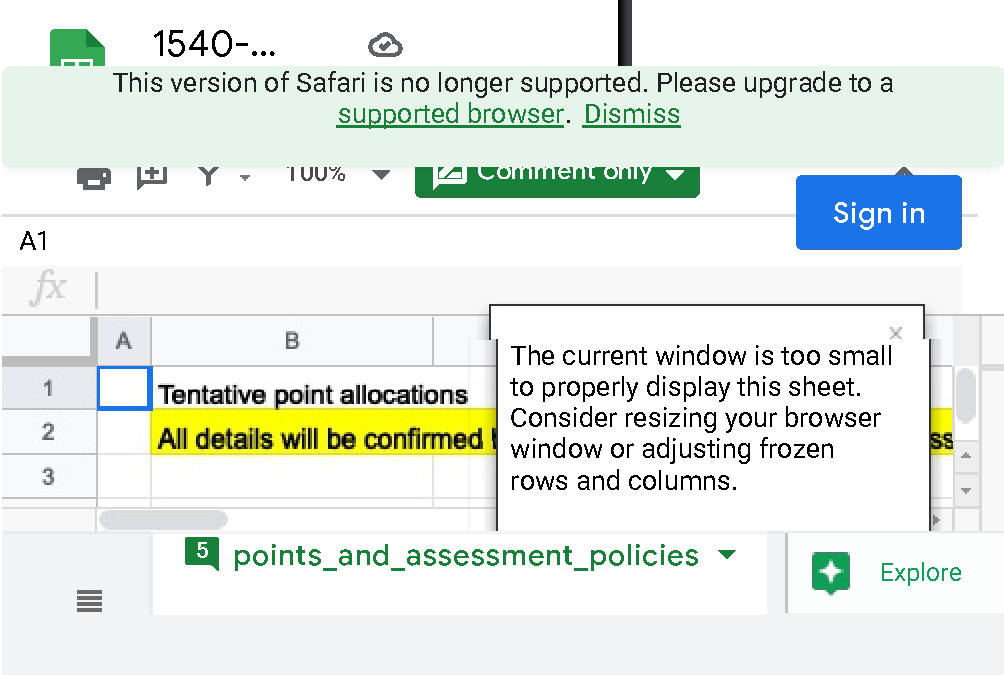
\includegraphics{1540_syllabus_files/figure-latex/unnamed-chunk-3-1.pdf}}

\hypertarget{semester-schedule}{%
\chapter{Semester schedule}\label{semester-schedule}}

The schedule of tests is available \href{https://docs.google.com/spreadsheets/d/1Zsqfqako3ctJByqRzbU2bTcv7fCXCKLHp_RDfzd-Qmg/edit?usp=sharing}{here}.

\href{https://docs.google.com/spreadsheets/d/1Zsqfqako3ctJByqRzbU2bTcv7fCXCKLHp_RDfzd-Qmg/edit?usp=sharing}{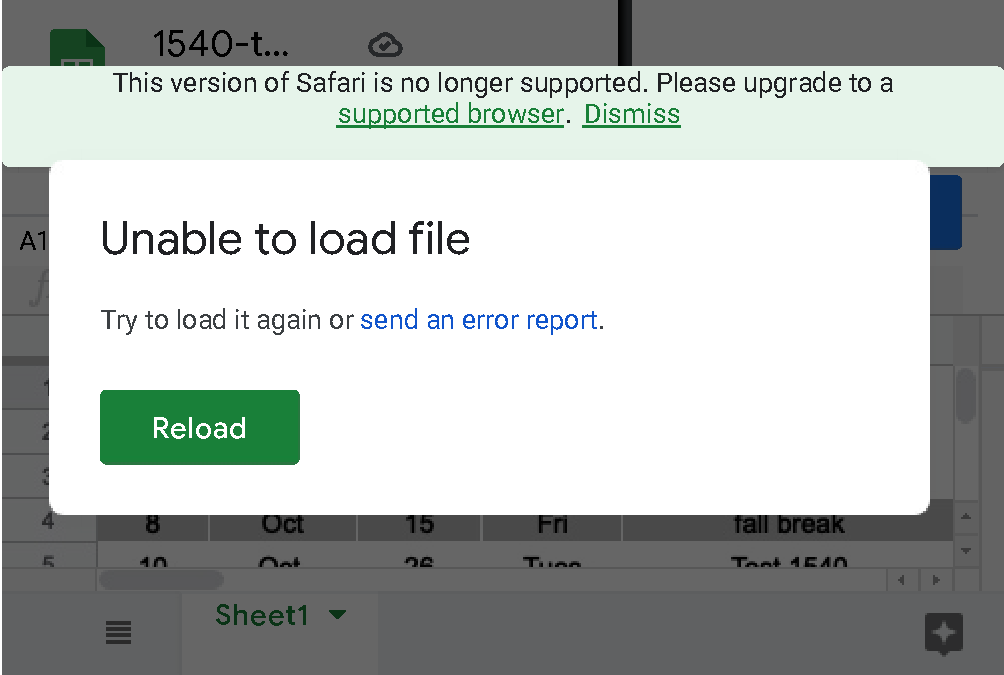
\includegraphics{1540_syllabus_files/figure-latex/unnamed-chunk-4-1.pdf}}

A calendar for the semester will be posted with key University dates and tests.

\hypertarget{weekly-schedule}{%
\chapter{Weekly schedule}\label{weekly-schedule}}

A summary of weekly events is available \href{https://docs.google.com/spreadsheets/d/12ryH_WBJadioURhMu9HHSO1NxyBA6f9QAuTdasXkY3Y/edit?usp=sharing}{here}. Commenting is enabled; feel free to post questions.

Each Friday I will send out an message via Canvas that will layout the topics and tasks for the following week.

\href{https://docs.google.com/spreadsheets/d/12ryH_WBJadioURhMu9HHSO1NxyBA6f9QAuTdasXkY3Y/edit?usp=sharing}{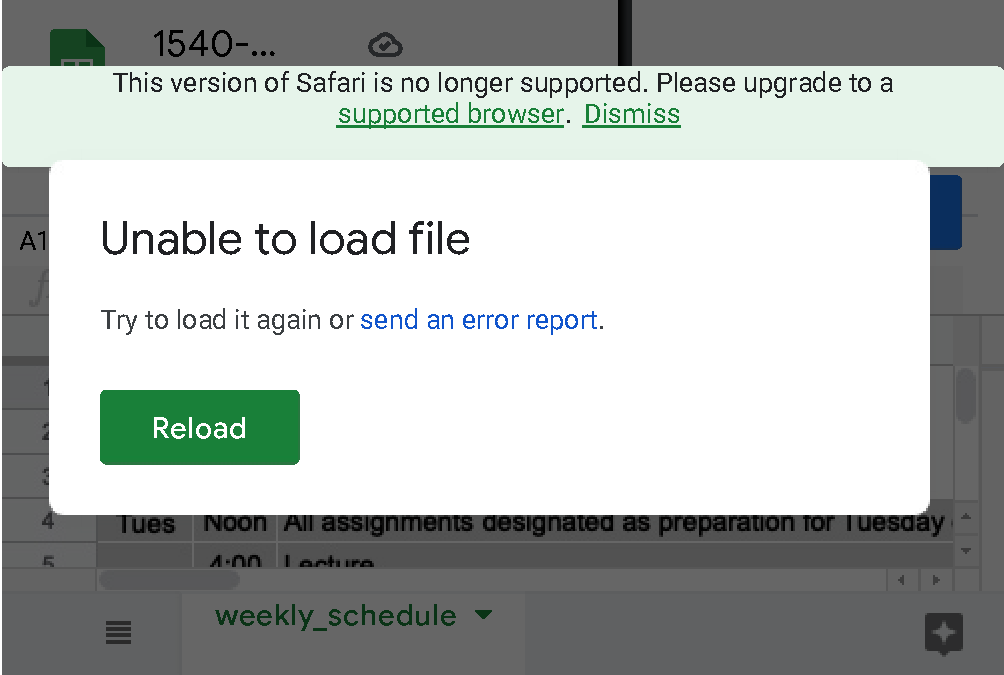
\includegraphics{1540_syllabus_files/figure-latex/unnamed-chunk-5-1.pdf}}

\hypertarget{tophat}{%
\chapter{TopHat}\label{tophat}}

We will use TopHat in-class and for homework. Please bring a charged TopHat compatible device to all lectures and recitations.

\href{www.tophat.com}{\textbf{TopHat}}\\
Join Code: \textbf{209015}\\
www.tophat.com

When logging into TopHat it will ask you for your university. Typing in ``University of Pittsburgh'' brings up 3 options: \textbf{select the first one} that just says ``University of Pittsburgh''.

\hypertarget{updates-to-schedule-syllabus}{%
\chapter{Updates to schedule \& syllabus}\label{updates-to-schedule-syllabus}}

I reserve the right to update the syllabus, schedule, point allocation and all other components of the course as necessary.

If changes occur after the first day of class, they will be clearly communicated in class and via email, and a revised syllabus and schedule distributed with major changes flagged.

\hypertarget{videos-of-lectures}{%
\chapter{Videos of lectures}\label{videos-of-lectures}}

The first two weeks of class lecture will be recorded using Zoom and posted to Panopto.

After the first lecture I will distribute the Panopto folder where the videos will be saved.

Note: Since this class is not meant to be taken asynchronously I will not actively support use of these videos.

\hypertarget{zoom}{%
\chapter{Zoom}\label{zoom}}

Class will be in-person and streamed live via Zoom the first two weeks.

\url{https://pitt.zoom.us/j/99372114800}\strut \\
Password: ``BLOSUM''

\hypertarget{appendix-graduate-school}{%
\chapter{Appendix: graduate school}\label{appendix-graduate-school}}

If you are considering graduate school you may wish to check out these resource:

So you want to go to graduate school?
O'Connel, Tim. ``A conversation about grad school'' \url{https://eatmorecookies.wordpress.com/2018/07/17/a-conversation-about-grad-school/}

Carson, W.P. 1999. A primer on how to apply and get admitted to graduate school in ecology and evolutionary biology. Bulletin of the Ecological Society of America 80(4):246-250. (PDF here: \url{https://sites.google.com/site/walterpagecarson/publications})

Stearns, S. Some modest advices for graduate students
Bulletin of the Ecological Society of America, 1987 - JSTOR
\url{https://stearnslab.yale.edu/some-modest-advice-graduate-students}

Thoughts on Stearns and Huey
Fox, J. 2015. Re-reading Stearns and Hueys some modest advice to gradate students.
\url{https://dynamicecology.wordpress.com/2015/09/08/rereading-stearns-and-hueys-some-modest-advice-to-graduate-students/}

On the publishing process: a tweet by \citet{dsquintana}
\url{https://twitter.com/dsquintana/status/1154820610750595072?s=20}

\hypertarget{cheat-sheets}{%
\chapter{Cheat sheets}\label{cheat-sheets}}

RStudio produces a number of \href{https://www.rstudio.com/resources/cheatsheets/\#ide}{cheatsheets}; the most useful ones for beginners are below.

\href{http://github.com/rstudio/cheatsheets/raw/master/base-r.pdf}{\textbf{Basic R code}}\\
\url{http://github.com/rstudio/cheatsheets/raw/master/base-r.pdf}

\textbf{RStudio}
\url{https://github.com/rstudio/cheatsheets/raw/master/rstudio-ide.pdf}

\textbf{RMarkdown}
\url{https://github.com/rstudio/cheatsheets/raw/master/rmarkdown-2.0.pdf}\\
\url{https://www.rstudio.com/wp-content/uploads/2015/03/rmarkdown-reference.pdf}

Translations of some of these cheat sheets can be found at the bottom of the RStudio page.

\hypertarget{appendix-getting-involved-in-computational-research}{%
\chapter{Appendix: Getting involved in (computational) research}\label{appendix-getting-involved-in-computational-research}}

Approaching a PI - A guide for undergraduates \url{https://thefemalescientist.com/guide/madeleine-hann/2053/approaching-a-pi-a-guide-for-undergraduates-in-stem/}

\hypertarget{shortcuts-in-r}{%
\chapter{Shortcuts in R}\label{shortcuts-in-r}}

Programmers are often obsessed with using keyboard shortcuts. You'll see me use some, and you might want to learn them.

The back of this cheatsheet is a 1-page summary of shortcuts
\url{https://github.com/rstudio/cheatsheets/raw/master/rstudio-ide.pdf}

Another summary sheet of Shortcuts in RStudio is here:
\url{https://support.rstudio.com/hc/en-us/articles/200711853-Keyboard-Shortcuts}

A great blog post on shortcuts is here
\url{https://appsilon.com/r-studio-shortcuts-and-tips/}

\end{document}
